\chapter{Gameplay}

\section{Menu}
Quando o jogo é iniciando é mostrado um menu.

\begin{figure}[h]
    \centering
    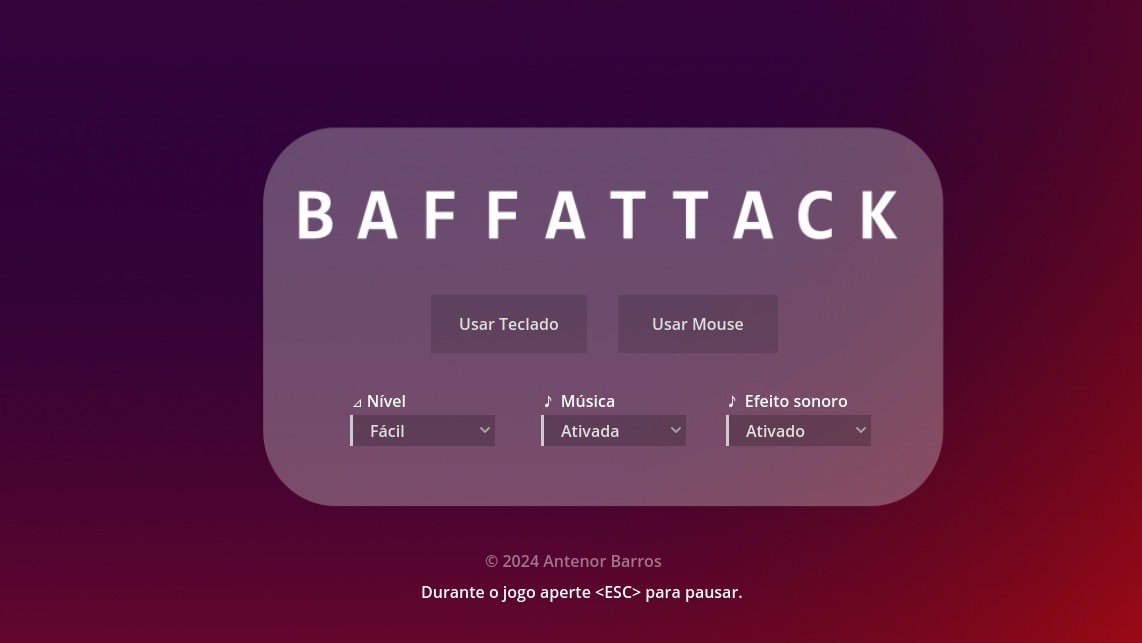
\includegraphics[width=\textwidth]{menu.png}
\end{figure}

Nele é possível escolher o nível de dificuldade, se a música de fundo estará ativa, se os efeitos sonoros estarão ativos e 
qual tipo de controle (teclado ou mouse) será usado.


\begin{figure}[h]
    \centering
    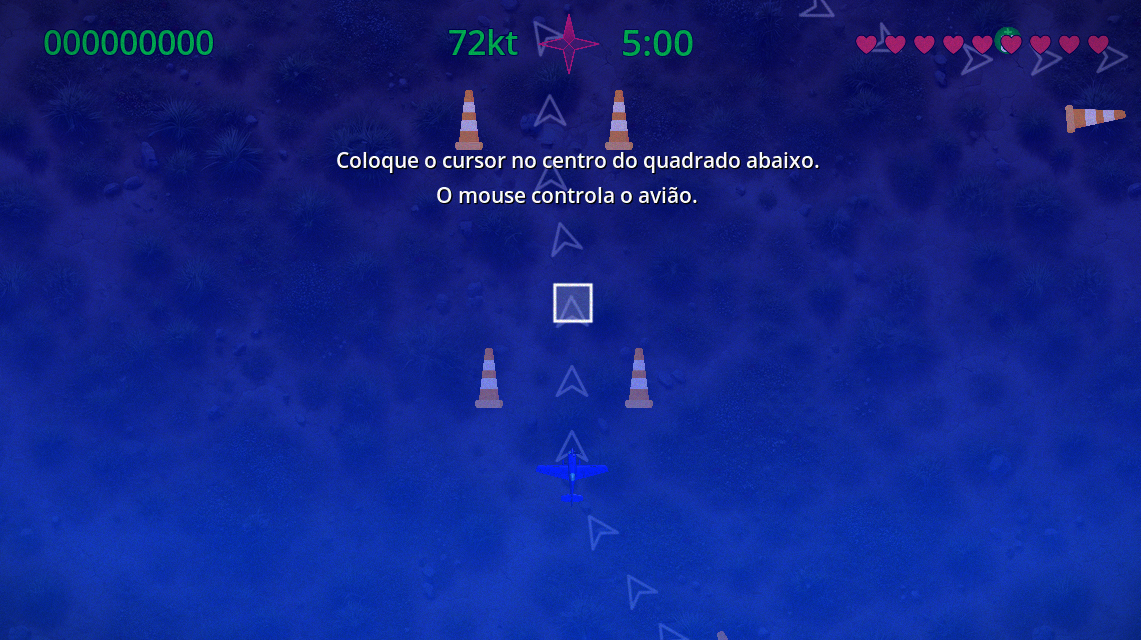
\includegraphics[width=\textwidth]{center.png}
\end{figure}

Na próxima tela o cursor deve ser centralizado no quadrado mostrado para o jogo se inicie.

\section{Jogo}

\begin{figure}[h]
    \centering
    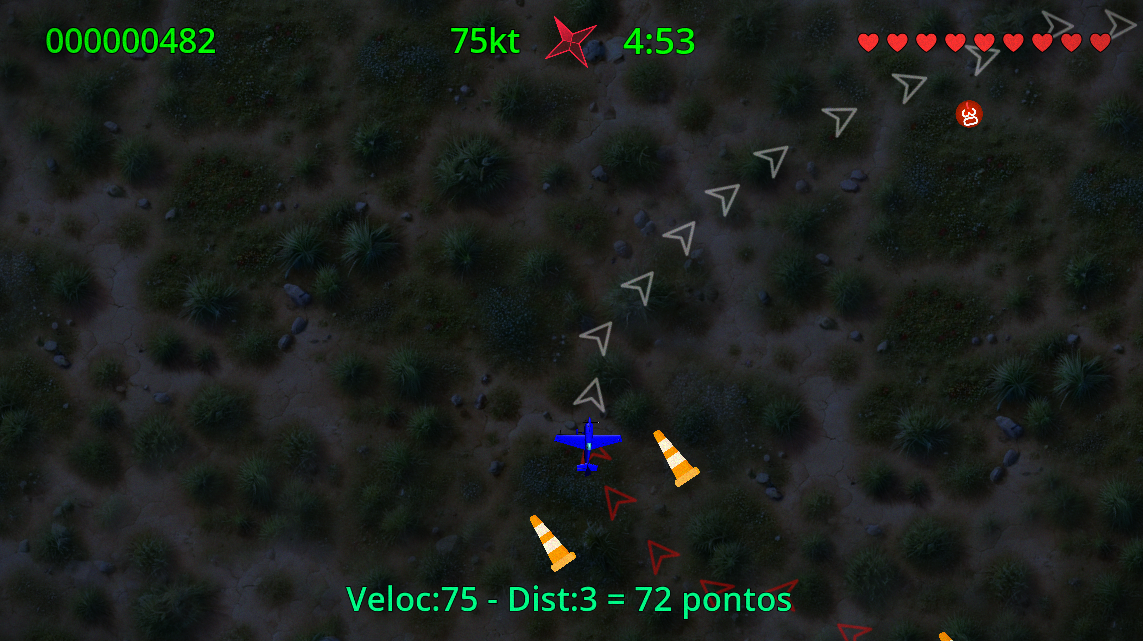
\includegraphics[width=\textwidth]{game.png}
\end{figure}

Na parte de cima do jogo aparece o HUD (head-up display) com as seguintes informações da
esquerda para direita:

\begin{itemize}
\item {Número de pontos}
\item {Velocidade do avião em nós (kt)}
\item {Rosa dos ventos para aumentar a consciência situacional}
\item {Tempo restante}
\item {Ícones de corações representando número de vidas restantes}
\end{itemize}

\chapter{Mecânica}

Como na corrida real, o avião deve passar pelos chamados "Air gates", que são duas colunas (pylon na Red Bull Air Race real) pelas quais a aeronave deve passar no meio, exigindo destreza e timing, já que nenhuma parte do avião pode tocar nas colunas. Na competição real, essas colunas são cones de nylon inflados com ar, como balões que não causam danos à aeronave em caso de colisão, apenas o material se rasga, indicando que o avião não passou corretamente.

\begin{figure}[h]
    \centering
    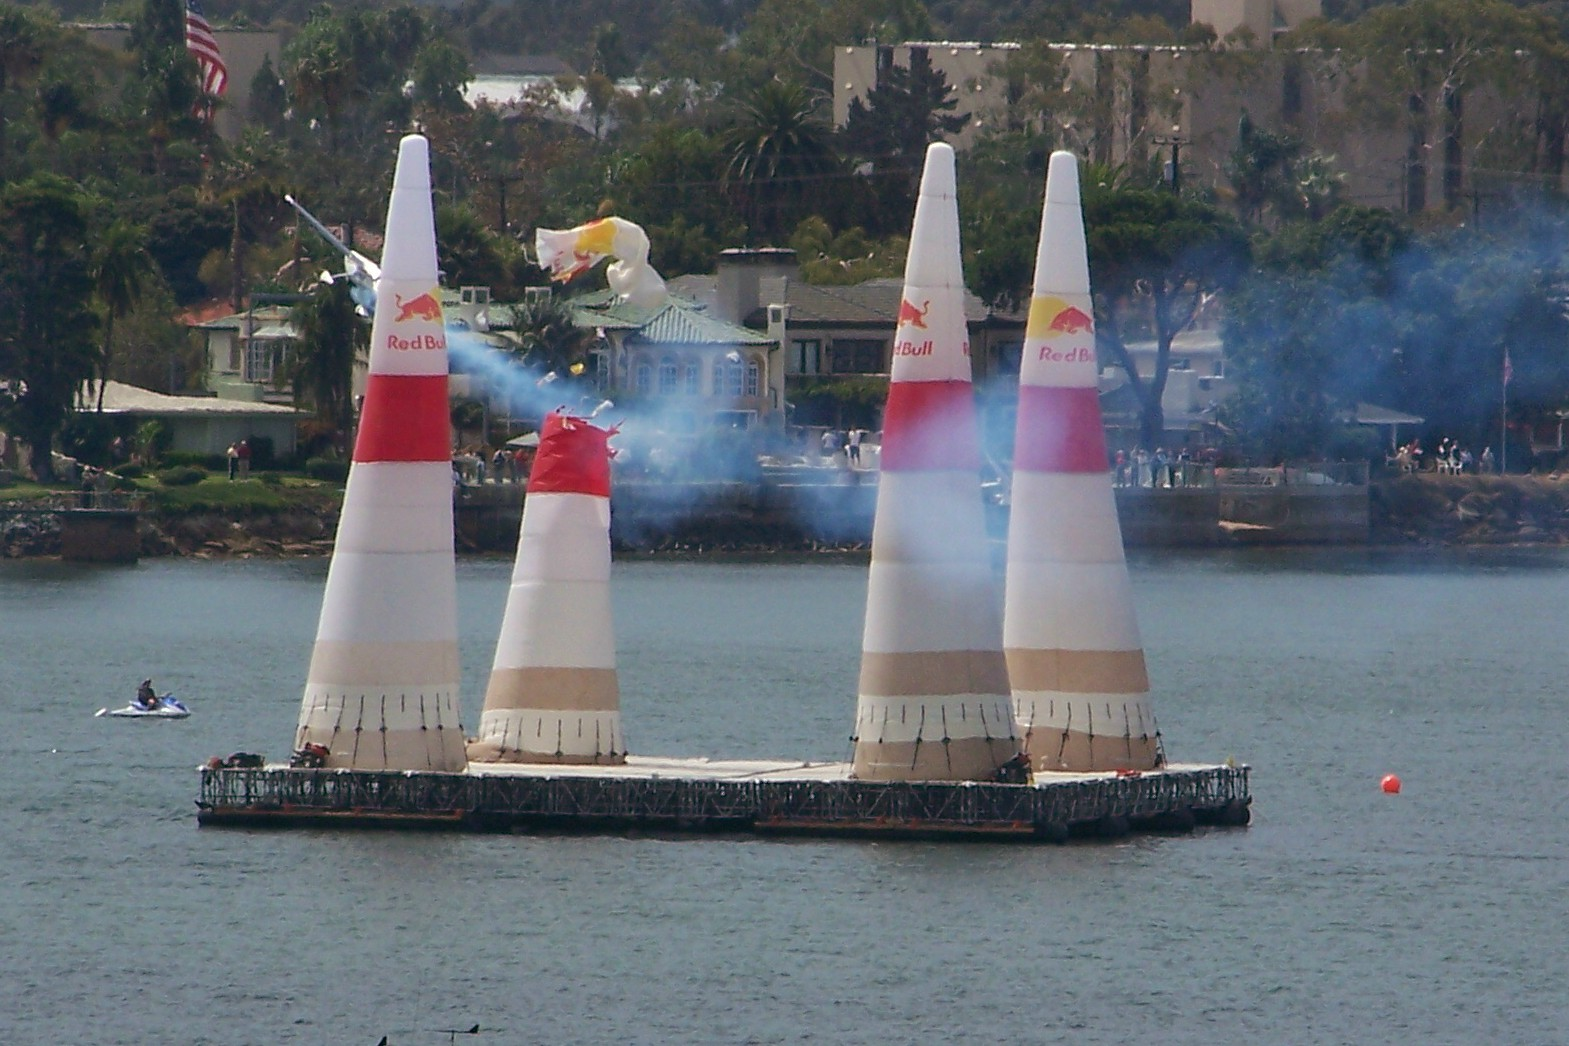
\includegraphics[width=0.8\textwidth]{red-bull-2.jpg}
\end{figure}

\section*{Air Gate}
Existem dois tipos de Air gates: o largo e o estreito.

\subsection*{Largo}
No largo, o avião deve passar sem tocar em nenhuma parte nas colunas. Caso toque, são descontados 100 pontos. Existe um sentido correto para passar; caso passe no sentido errado, são perdidos 500 pontos.

\subsection*{Estreito}
No Air gate estreito, as regras anteriores também valem, mas uma dificuldade extra é adicionada. Quando estiver passando, o avião deve estar com as asas inclinadas, mais precisamente com \texttt{abs(R) >= R\_max / 2}. O significado de \texttt{R} e \texttt{R\_max} foi explicado anteriormente. 
Caso esta regra seja descumprida, são descontados 50 pontos. O desconto é cumulativo, então, caso o avião passe em voo nivelado e atinja um dos cones, são perdidos 150 pontos.

\section*{Power up/down}
O jogo dura 5 minutos, mas aparecem em posições aleatórias do mapa "power-ups" de tempos que dão 30 segundos extras caso o avião passe por cima de um. 
Este possui a cor verde. Caso esteja na cor vermelha é descontado 1 minuto. Ambos os power-ups desaparecem ao serem passados.

\section*{ExtraHealth}
Existe também um power up que, caso o avião atravesse-o, é dada uma vida extra.

\section*{Caminho}
O avião deve seguir a ordem de "airgates" mantendo-se dentro de um caminho pre-estabelecido. A cada delta, a distância do avião ao caminho é calculada. A partir de um limiar, o jogador começa a perder ponto em uma razão proporcional à distância do caminho. Caso ele fique muito longe, em poucos segundos seu escore chega a zero e ele perde.

\section*{Término do jogo}
O jogo termina se uma ou mais destas condições ocorrerem:
\begin{enumerate}
    \item O tempo chegar em zero;
    \item Os pontos do jogador ficarem iguais a zero ou negativos.
\end{enumerate}

